\chapter{Comparative Analysis and Conclusion}
\label{cp:conclusion}

\section{The Linear vs. Tree Gap: A Question of Interactions}
\label{sec:gap}
The comparative analysis revealed a stark performance gap between the Linear models ($\text{MCC} \approx 0.54$) and the Tree-based models ($\text{MCC} \approx 0.65$).
\begin{itemize}
    \item \textbf{The "Additive" Limitation}: Despite extensive feature engineering (binning non-linear features), Linear models still plateaued. This confirmed that the primary challenge was not the shape of individual variables, but the presence of \textbf{complex conditional interactions} (e.g., between \texttt{Age}, \texttt{Education}, and \texttt{Marital Status}).
    \item \textbf{Tree Superiority}: Decision tree ensembles naturally capture these high-order interactions through their hierarchical structure, resulting in a crucial $\mathbf{+11}$ point jump in $\text{MCC}$.
\end{itemize}

\vspace{1 \baselineskip}
\section{Comparison of Boosting Models Results}
\label{sec:comparison}
The top-tier boosting algorithms (Meta Models) converged toward a similar optimal solution, with the GradientBoostingClassifier edging out the competition:

\begin{table}[H]
    \centering
    \caption{Top Model Performance on Test Set}
    \begin{tabular}{||l|c|c|c||}
        \hline
        \textbf{Model} & \textbf{MCC} & \textbf{Recall ($>\$50$K)} & \textbf{Precision ($>\$50$K)} \\
        \hline
        \textbf{GBClassifier} & \textbf{0.6477} & \textbf{0.66} & 0.79 \\
        LightGBM/XGBoost & $0.645$ & $0.65$ & $0.80$ \\
        CatBoost & 0.638 & 0.64 & 0.78 \\
        \hline
    \end{tabular}
\end{table}

\vspace{1 \baselineskip}
\section{Final Model Selection and Justification}

The \textbf{GradientBoostingClassifier} was selected as the final model. We tested SMOTE to rebalance the dataset, but it slightly lowered our MCC, so we decided not to include it in the final version.

Using SMOTE also changed the model’s behavior: it started predicting the “>50K” class more often, but at too high a cost. For every correctly identified high-income individual, the model misclassified more than one low-income individual. Since we do not prioritize one class over the other, this trade-off is not beneficial—and this is clearly reflected in the MCC.


\begin{itemize}
    \item \textbf{Performance}: It secured the top performance metrics (Best $\text{MCC}$) and demonstrated the highest ability to detect high-income individuals (Best Recall of $0.66$) among the top-tier models.
    \item \textbf{Suitability}: It successfully leveraged the complex, non-linear interactions within the census data that were not accessible to the baseline models.
\end{itemize}



\section{Feature Importance: Drivers of Income Inequality}
\label{sec:feature_importance}

Performance analysis is crucial, but for the business case, understanding the primary drivers is equally important. Using the $\text{XGBoost}$ model's gain metrics, we identified the most influential socioeconomic factors in predicting high income. The top 10 features are visualized below, with the magnitude of the importance score corresponding to the feature's utility in the tree ensemble model. 

\begin{figure}[H]
    \centering
    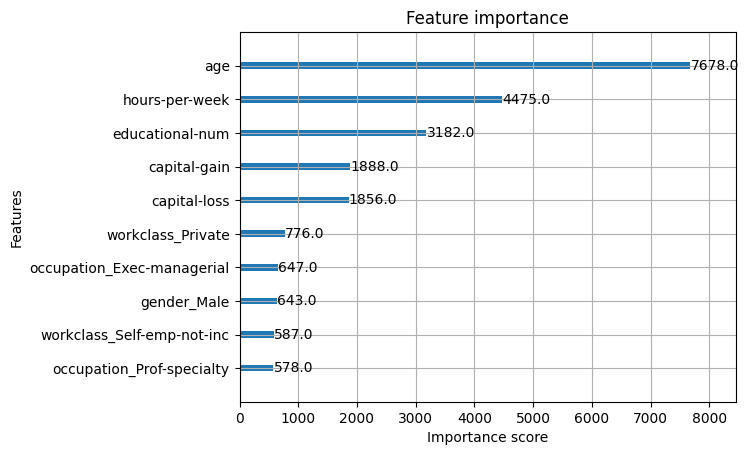
\includegraphics[width=0.9\textwidth]{Images/feature_importance.png} 
    \caption{Importance of the 10 most useful features, based on XGBoost gain metrics. }
    \label{fig:feature_importance}
\end{figure}

The analysis confirms that the \textbf{Age} (the single strongest predictor, confirming the importance of life stage/experience), \textbf{Hours-per-week}, and \textbf{Educational-num} are the central drivers. Furthermore, the high ranking of the engineered $\texttt{capital-gain}$ and $\texttt{capital-loss}$ features reinforces our decision to treat capital events as a proxy for wealth/market participation.

\vspace{1 \baselineskip}




\section{Conclusion on how the Business Case was Addressed}
\label{sec:business_case}

Our project successfully determined the most influential factors for income prediction, as detailed in Section \ref{sec:feature_importance}. By using a relevant Feature Engineering strategy and employing a high-performing ensemble model, we created a predictive system (Gradient Boosting Classifier, $\text{MCC}=0.6477$) that is both highly accurate and mathematically honest about the significant class imbalance. This model allows a business or policy analyst to assess the probability of an individual earning over $\$50\text{K}$ based on these demographic and employment factors with a high degree of confidence, directly fulfilling the initial business objective of identifying high-potential segments.


\vspace{2 \baselineskip}